\documentclass[paper=a4, fontsize=11pt]{scrartcl}
\usepackage{amsmath,amsfonts,amsthm}
\usepackage{graphicx}
\usepackage{multirow}
\usepackage{hhline}
\usepackage{parskip}
\usepackage{hyperref}
\usepackage{chngcntr}

\newcommand{\horrule}[1]{\rule{\linewidth}{#1}}
\parskip = \baselineskip

\title{
	\normalfont \normalsize \textsc{THE PENNSYLVANIA STATE UNIVERSITY} \\ [25pt]
	\horrule{1pt} \\[0.4cm]
	\huge {\bf CSE585/EE555: Digital Image Processing II Report 2 \\ Mathematical Morphology} \\
	\horrule{2pt} \\[0.5cm]
}
\author{
	\normalfont \normalsize
	 Wei-Kai Su, Yu-Hsuan Kuo\\[-3pt] \normalsize
  \today
}
\date{}

\begin{document}
\maketitle

\section{Objectives}
This project is mainly focus on (1)Tall-Character Recognition. (2) Morphological Skeleton. (3) Shape Analysis. The objectives of this project 1 are listed as follows: 

\begin{itemize}
	\item applying the conditional dilation to detect Tall-Character.
	\item implementing the morphological skeleton algorithm, and partial reconstruction.
	\item find the minimum bounding rectangle, and calculate size distribution, pectrum, and complexity to recognize the best matches.

\end{itemize}




\section{Tall-Character Recognitions}
The goal is to extract the "tall"(elongated) characters in the image, where the tall characters (e.g., "H", "p", and "l") roughly have height $\geq$ 18 pixels, and the short characters (e.g., "e") roughly have height $\leq$ 14 pixels. We did the thresholding in the first step before applying the morphological operations. For those pixel value that are larger than 20, we reset the pixel value to 1, and we reset the pixel value to 0 for those with pixel value smaller than 20.  After thresholding, the image becomes a binary image. 

Furthermore, we used the method in L5-4 of the lecture notes.  Let  $X_0 = X_B$, and we applied opening method to $X$, the input image, by using structuring element $B$ of size 18 $\times$ 1 pixels. This is because those characters which are taller than or equal to 18 will remain in the image after opening method.  Figure \ref{fig:1} demonstrates the result of $X_0$.
Next, we performed the Conditional Dilation for $X_i$. The formula is $X_i = (X_{i-1} \oplus B') \cap X$ for $i = 1,2, \dots $ until $X_i = X_{i-1}$. The structuring element B' is different from the structuring element B, and B' is 3 by 3 square. The figure \ref{fig:2}, \ref{fig:3}, \ref{fig:4}, \ref{fig:5} shows the steps to the final result in the figure \ref{fig:6}.
 
The detailed implementation is shown in the $main1.m $ file. 


\begin{figure}
	\centering
	
\includegraphics[width=11cm]{Q1_X0.eps}
	\caption{$X_0 = X_B$.}
	\label{fig:1}
\end{figure}


\begin{figure}
	\centering
	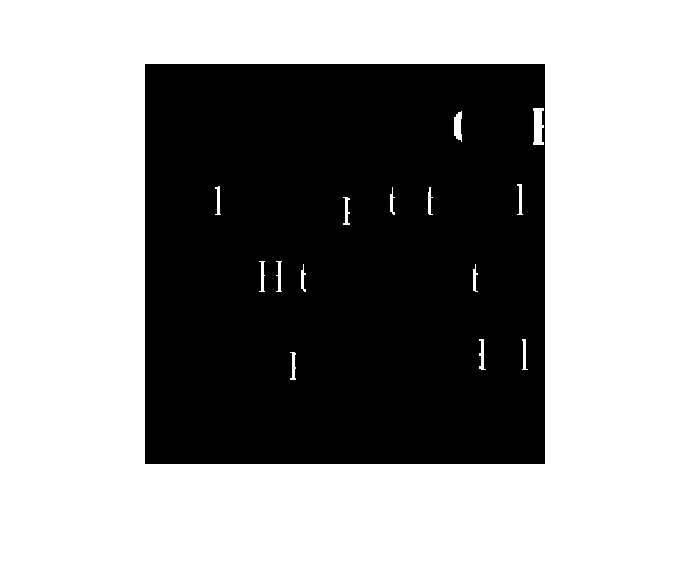
\includegraphics[width=11cm]{Q1_X1.eps}
	\caption{$X_1$.}
	\label{fig:2}
\end{figure}

\begin{figure}
	\centering
	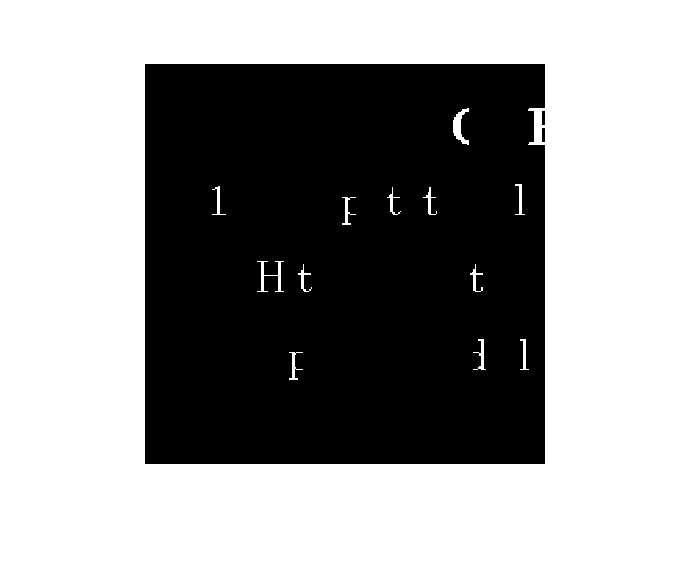
\includegraphics[width=11cm]{Q1_X5.eps}
	\caption{$X_5$.}
	\label{fig:3}
\end{figure}

\begin{figure}
	\centering
	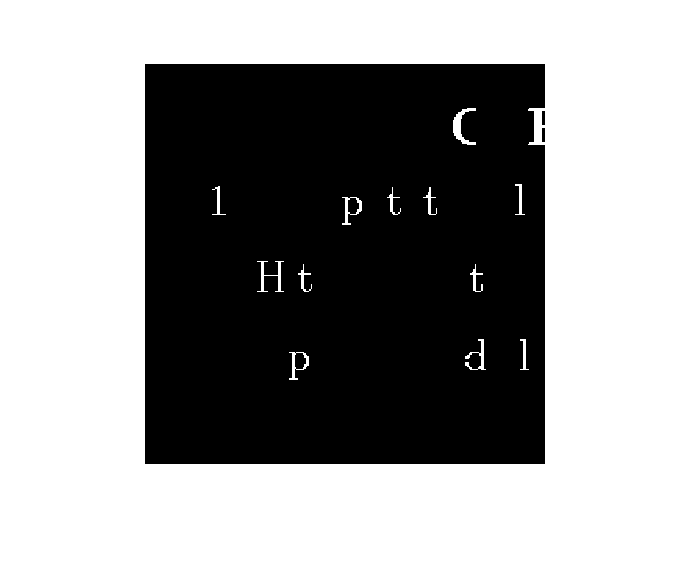
\includegraphics[width=11cm]{Q1_X10.eps}
	\caption{$X_{10}$.}
	\label{fig:4}
\end{figure}

\begin{figure}
	\centering
	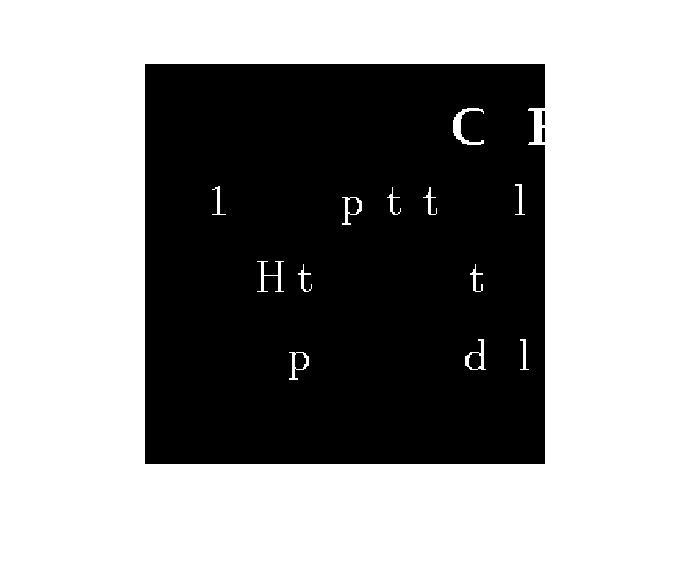
\includegraphics[width=11cm]{Q1_X15.eps}
	\caption{$X_{15}$.}
	\label{fig:5}
\end{figure}

\begin{figure}
	\centering
	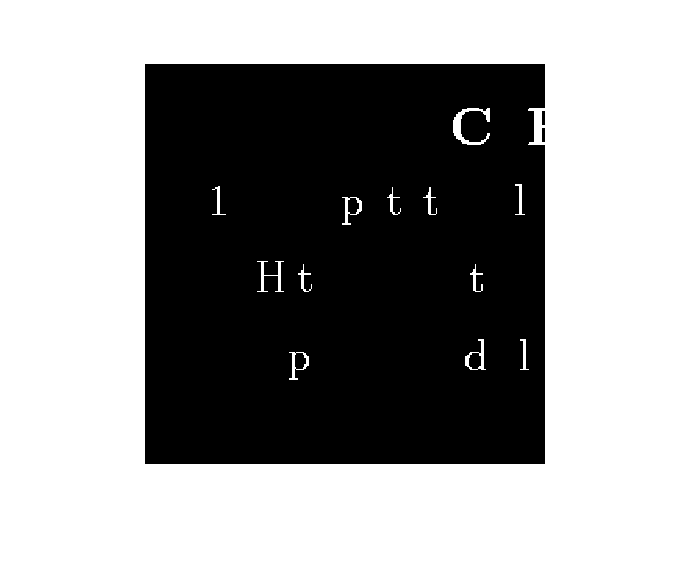
\includegraphics[width=11cm]{Q1_X20.eps}
	\caption{Tall-Character Final Result : $X_{20}$.}
	\label{fig:6}
\end{figure}






\section{Morphological Skeleton}

We used the method in L6-1 of lecture notes : $sk(X) = \cup_{0 \leq n \leq N} S_n(X)$, where $S_n(X) = (X \ominus nB) - (X \ominus nB)_B$, and $S_0(X) = X - X_B$. The structuring element B is a 3 by 3 square. We applied this algorithm to the "bear" image and the "penn256" image. Figure \ref{fig:7} and \ref{fig:8} demonstrate the result of morphological skeleton. 

Next, we applied the formula in L6-2 of lecture notes : $X_{kB} =  \cup_{k \leq n \leq N} [ S_n(X) \oplus nB ] $, where $k \geq 0$. The result of  partial reconstructions $X_{2B}$, $X_{3B}$, and $X_{4B}$ for "bear" image is presented in figure  \ref{fig:9},  \ref{fig:10}, and  \ref{fig:11}. As for the "penn256" image, figure  \ref{fig:12},  \ref{fig:13}, and  \ref{fig:14} presents the partial reconstructions $X_{2B}$, $X_{3B}$, and $X_{4B}$ respectively.


The detailed implementation of Morphological Skeleton is shown in the $main2.m $ file and the detailed implementation of partially reconstruction is shown in the $part_Reconstruct.m$ file. 

\begin{figure}
	\centering
	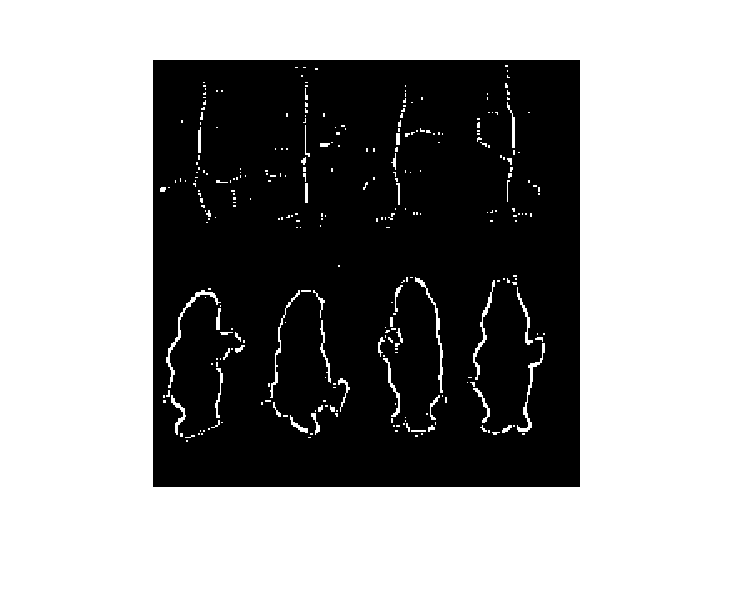
\includegraphics[width=11cm]{SKbear.eps}
	\caption{Morphological Skeleton of bear .}
	\label{fig:7}
\end{figure}

\begin{figure}
	\centering
	
\includegraphics[width=11cm]{skpenn.eps}
	\caption{Morphological Skeleton of penn256 .}
	\label{fig:8}
\end{figure}


\begin{figure}
	\centering
	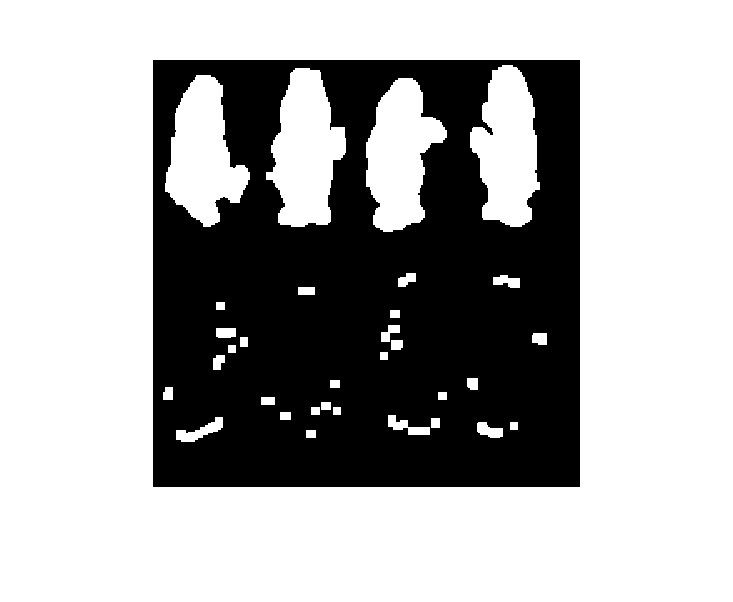
\includegraphics[width=11cm]{X2Bbear.eps}
	\caption{Partial Reconstructions $X_{2B}$ of bear image.}
	\label{fig:9}
\end{figure}

\begin{figure}
	\centering
	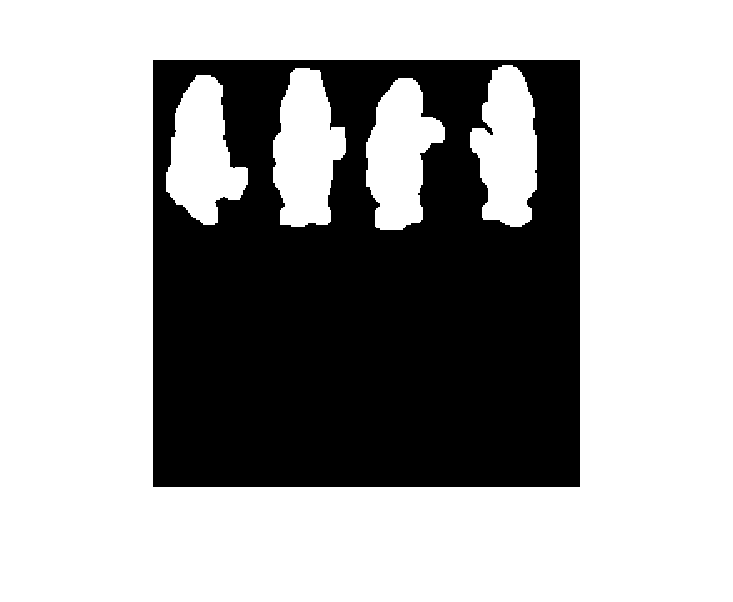
\includegraphics[width=11cm]{X3Bbear.eps}
	\caption{Partial Reconstructions $X_{3B}$ of bear image.}
	\label{fig:10}
\end{figure}

\begin{figure}
	\centering
	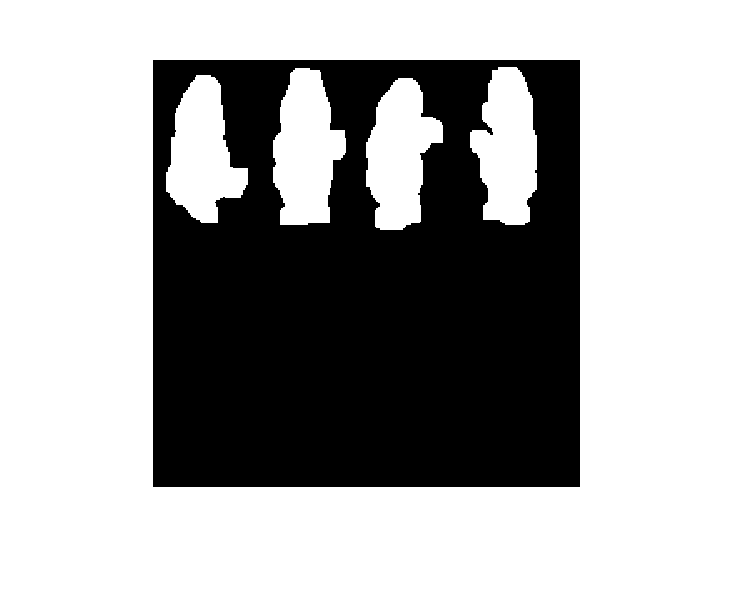
\includegraphics[width=11cm]{X4Bbear.eps}
	\caption{Partial Reconstructions $X_{4B}$ of bear image.}
	\label{fig:11}
\end{figure}



\begin{figure}
	\centering
	
\includegraphics[width=11cm]{X2Bpenn.eps}
	\caption{Partial Reconstructions $X_{2B}$ of penn256 image.}
	\label{fig:12}
\end{figure}

\begin{figure}
	\centering
	
\includegraphics[width=11cm]{X3Bpenn.eps}
	\caption{Partial Reconstructions $X_{3B}$ of penn256 image.}
	\label{fig:13}
\end{figure}

\begin{figure}
	\centering
	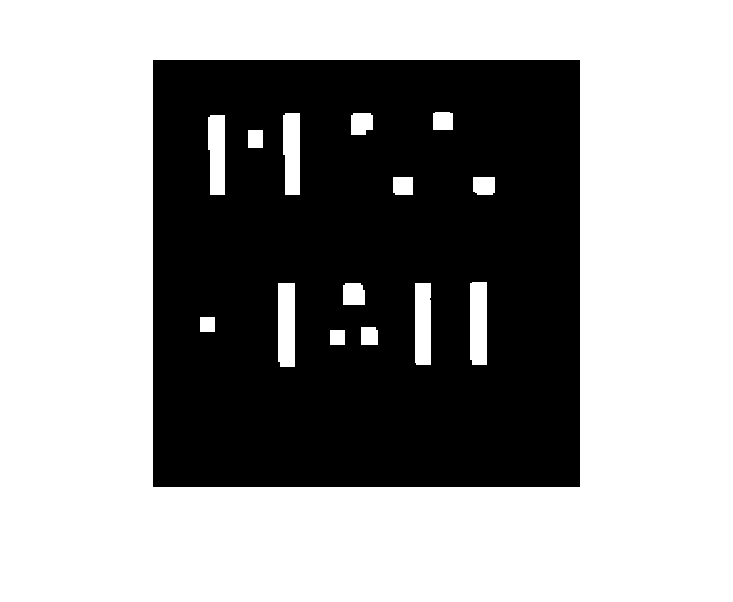
\includegraphics[width=11cm]{X4Bpenn.eps}
	\caption{Partial Reconstructions $X_{4B}$ of penn256 image.}
	\label{fig:14}
\end{figure}


\section{Shape Analysis}

\subsection{ Method For Part (a) }

First, we found minimum boundary rectangles in "match1" image for each object: clover, spade, steer, and airplane. We implemented this operation in $minbounrec.m$ file : we used build-in functions : bwconncomp and labelmatrix, and divided the whole image to four different labeled regions.  Also, We defined these four regions as four distinct objects. 

	Second, we used the formulas in L6-11 to L6-15 to calculated size distribution, pattern spectrum and shape complexity. The corresponding implementations are shown in $sizedistr.m$, $Pecstrum.m$ and $shapcomplx.m$, respectively. In addition, we found the most complex object in match1 is airplane because of its highest shape complexity value.

	Third, we implemented the method described in L6-15 to decide what is best matching objects in "match3"  for objects in "match1". These operation is realized in $bestmatch1.m$ file.  Moreover, we set all elements to 1 in C.
\subsection{ Result }

The results are shown in the figure \ref{fig:15} to figure \ref{fig:22}.
 
\begin{figure}
	\centering
	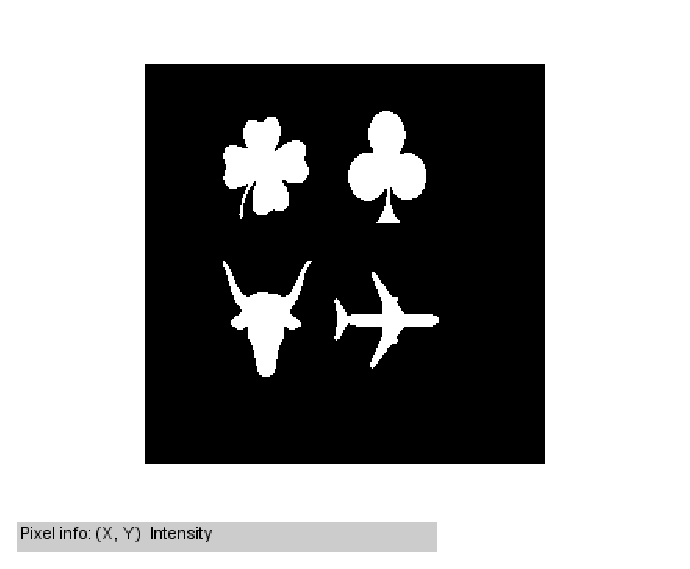
\includegraphics[width=11cm]{match1.eps}
	\caption{"Match1" image}
	\label{fig:15}
\end{figure}

\begin{figure}
	\centering
	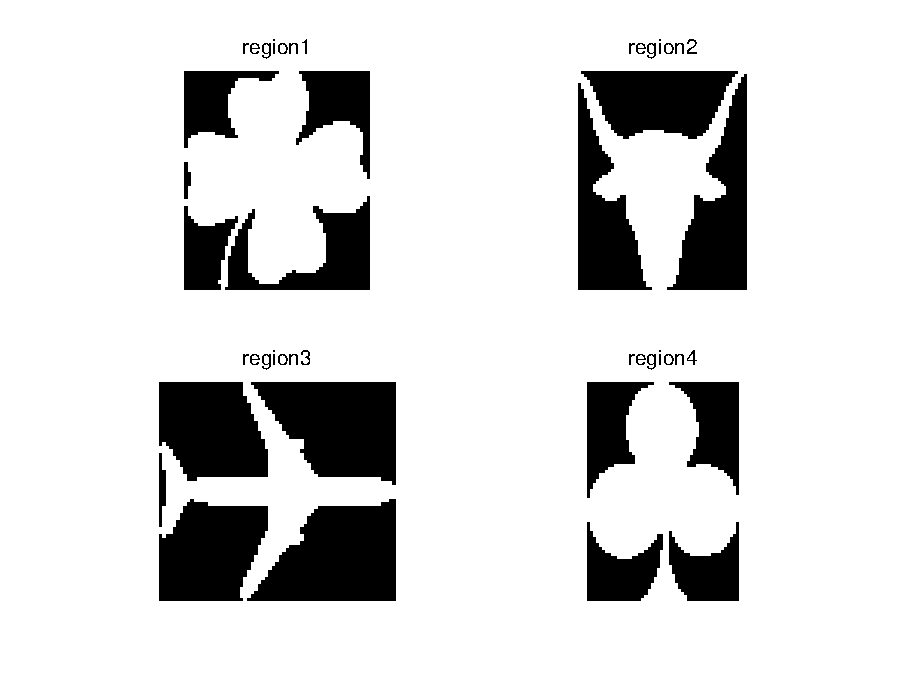
\includegraphics[width=11cm]{original4object.eps}
	\caption{Four Objects in "Match1". }
	\label{fig:16}
\end{figure}

\begin{figure}
	\centering
	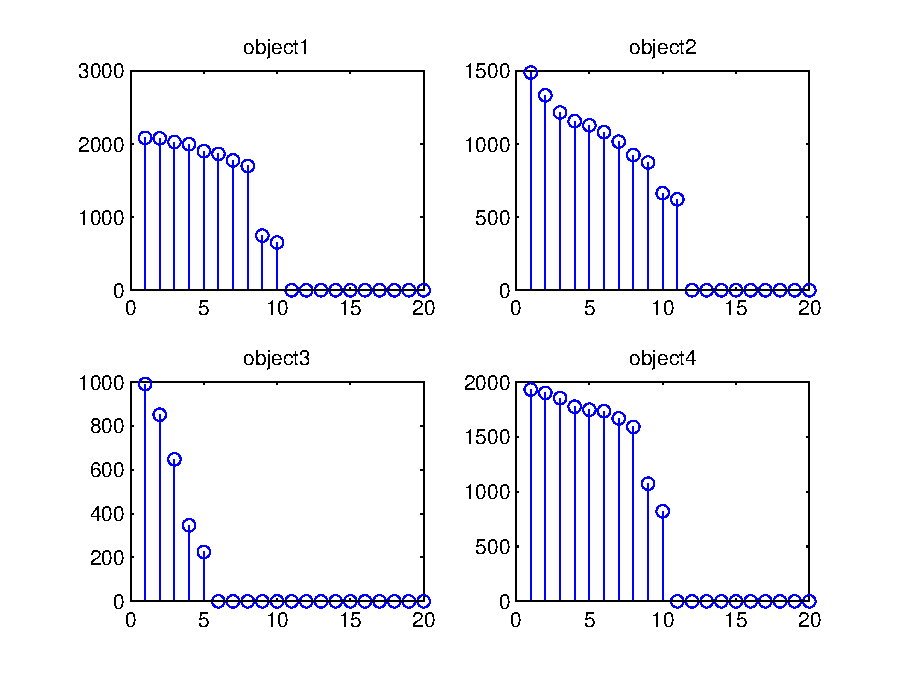
\includegraphics[width=11cm]{size_distribution_for_4object.eps}
	\caption{Size Distribution For Four Objects in "Match1". }
	\label{fig:17}
\end{figure}




\begin{figure}
	\centering
	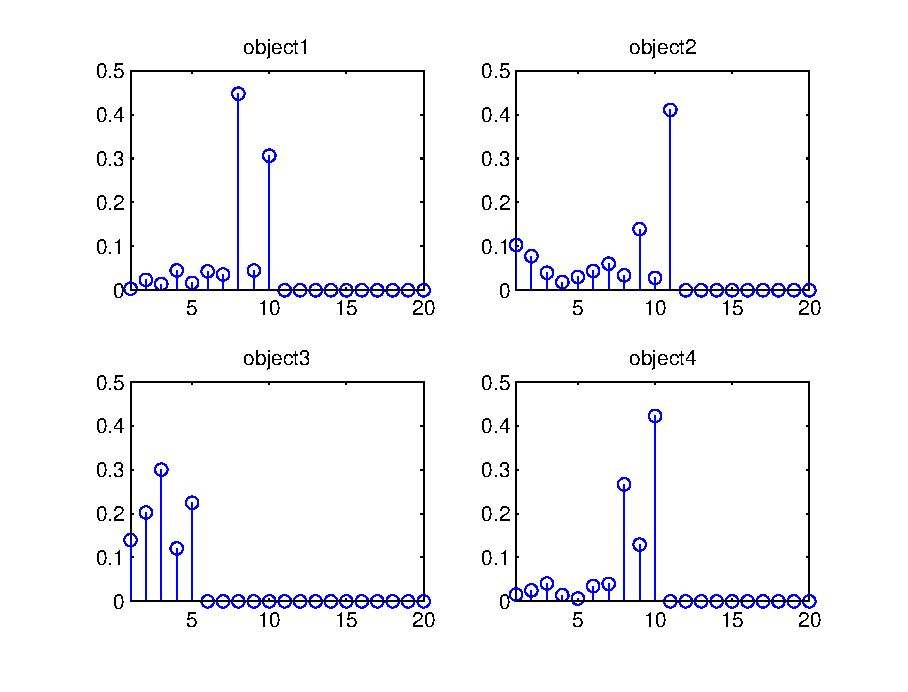
\includegraphics[width=11cm]{pecstrum_for_4object.eps}
	\caption{Pectrum for Four objects in "Match1".  }
	\label{fig:18}
\end{figure}


\begin{figure}
	\centering
	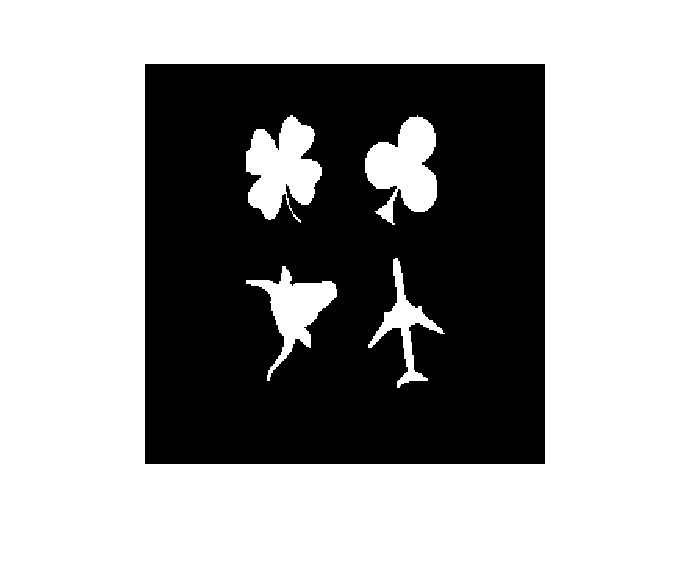
\includegraphics[width=11cm]{match3.eps}
	\caption{ "Match3" image. }
	\label{fig:19}
\end{figure}

\begin{figure}
	\centering
	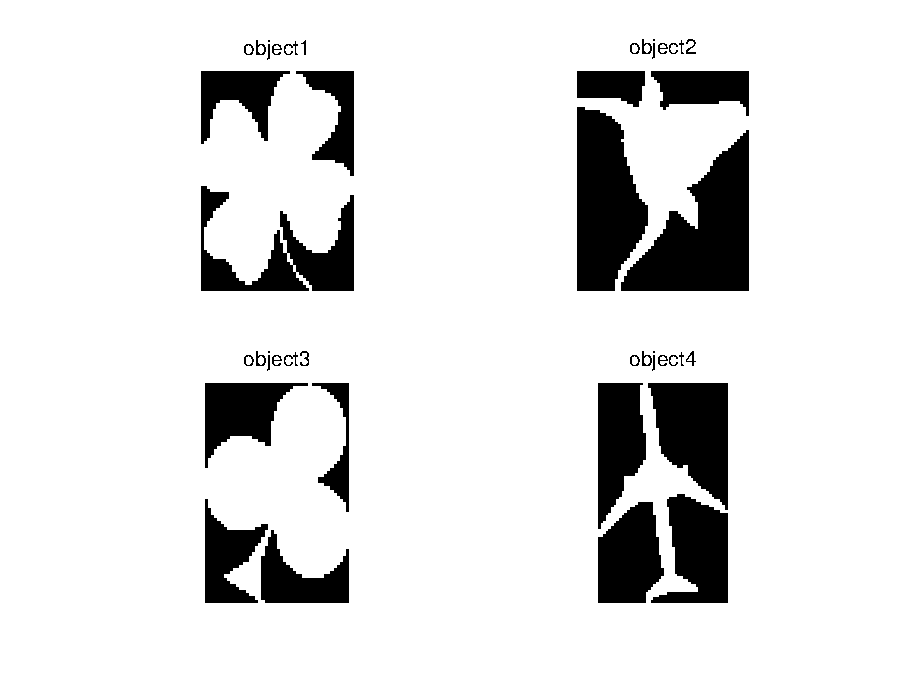
\includegraphics[width=11cm]{rotated_4object.eps}
	\caption{ Four Rotated Objects in "match3". }
	\label{fig:20}
\end{figure}




\begin{figure}
	\centering
	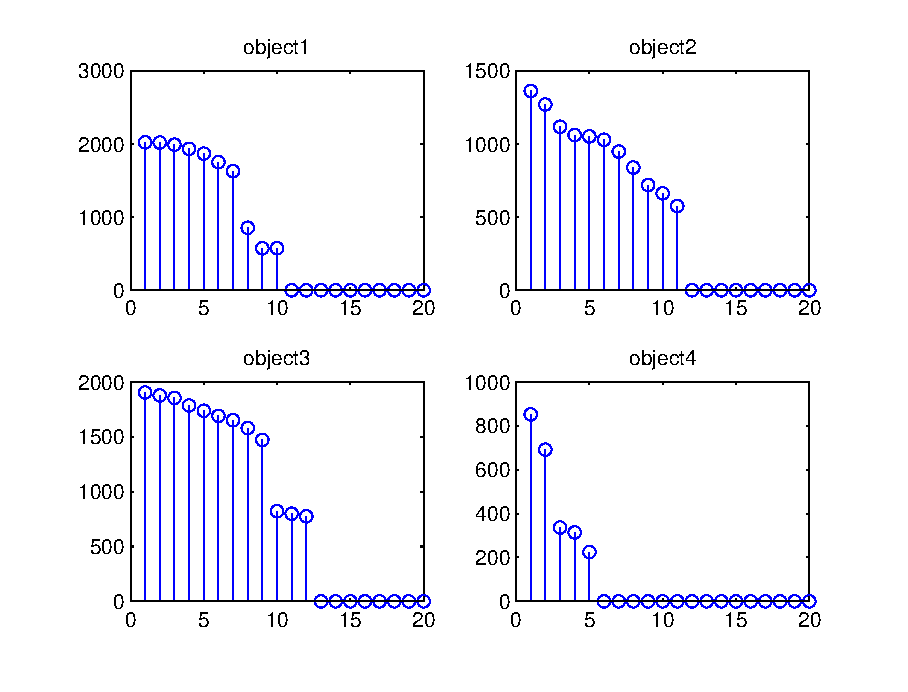
\includegraphics[width=11cm]{size_distribution_for_rotaterd_4object.eps}
	\caption{Size Distribution For Four Rotated Objects in "Match3". }
	\label{fig:21}
\end{figure}

\begin{figure}
	\centering
	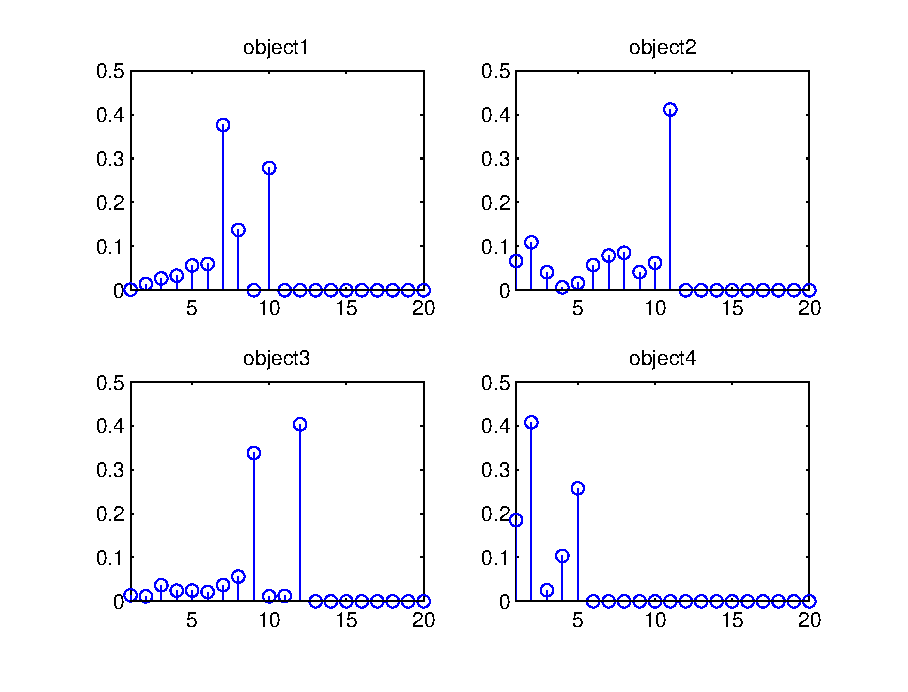
\includegraphics[width=11cm]{pecstrum_for_rotated_4object.eps}
	\caption{Pectrum for Four objects in "Match3". }
	\label{fig:22}
\end{figure}






\subsection{ Discussion }

	However, there is a very special phenomenon that the matched results have some overlapped. That is, there is one object (steer) in "match1" which is matched by two objects (steer, spade) in "match3".  In order to resolve this problem, we observed the pectrum of "match1" and "match3", and we set C(1)~C(6) equal to 1, and the other element in C are set to zero. By doing so, we got a perfect matching! To put another word,







\subsection{ Method For Part (b) }


In problem 3.(b), since we just have to identify four solid objects in "shadow1" image to corresponding objects in "shadow1rotated" image, we applied the conditional dilation method we used in the first problem to remove the hollow objects in these two images: 
	First, from observing both hollow and solid objects, we can choose a structuring element B1 (pixels 25 by 5),through opening original images ( "shadow1" image and "shadow1rotated1" image ), and removed hollow object, which thickness are less than 25 by 5, and kept some part of solid ones.
	Second, using the dilation of previous result by structuring element B2 of size 5 by 5, we got the image which only remained these four solid objects. The reason why we chose B2 is that a square structuring object can dilate a image in 8-direction: left, right, upper, lower, and two diagonal directions. In addition, the structuring element B2 of size 5 by 5 can reconstruct the solid objects more quickly than a 3 by 3 structuring element in both "shadow1" image and "shadow1rotated1" image.
	 
	After getting solid objects, we started to match the objects in "shadow1" and the objects in "shadow1rotated". The process is as follows: First, as mentioned before, we used the method stated in L6-15 to find a best matched objects of objects in "shadow1rotated" from the objects in "shadow1". In other words, we calculated the distance between objects in "shadow1" and objects in "shadow1rotated" to decide the best match. 
 	 
	
\subsection{ Result }

\begin{figure}
	\centering
	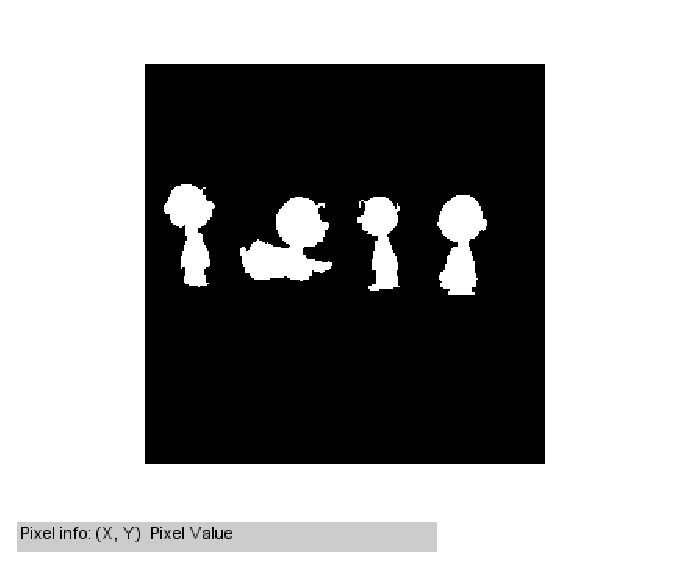
\includegraphics[width=11cm]{shadow1_solidpart.eps}
	\caption{Solid Objects in "shadow1" image. }
	\label{fig:23}
\end{figure}

\begin{figure}
	\centering
	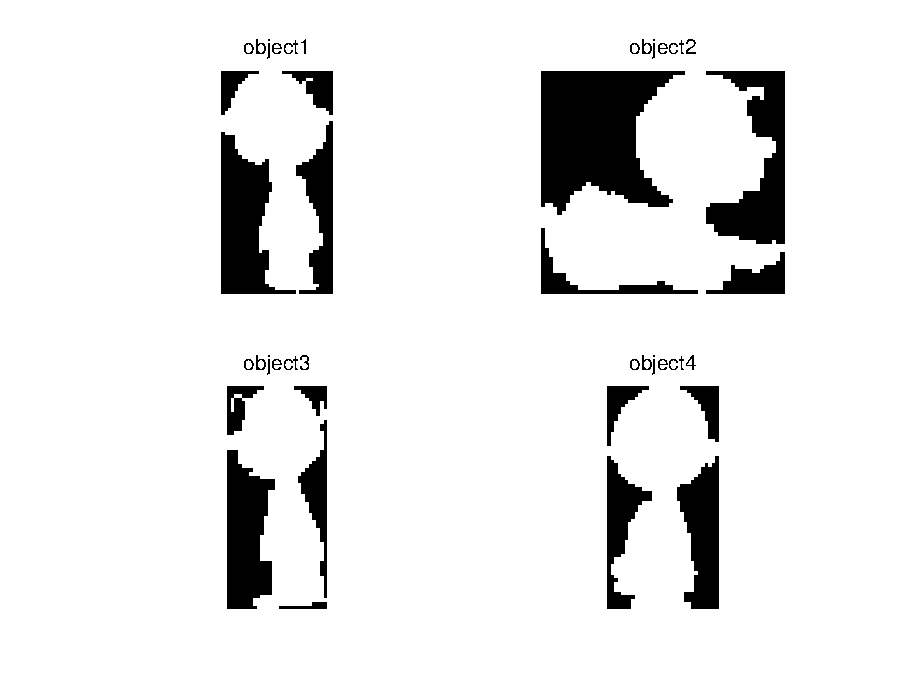
\includegraphics[width=11cm]{4objectinshadow1.eps}
	\caption{ Four Objects in "shadow1" image. }
	\label{fig:24}
\end{figure}

\begin{figure}
	\centering
	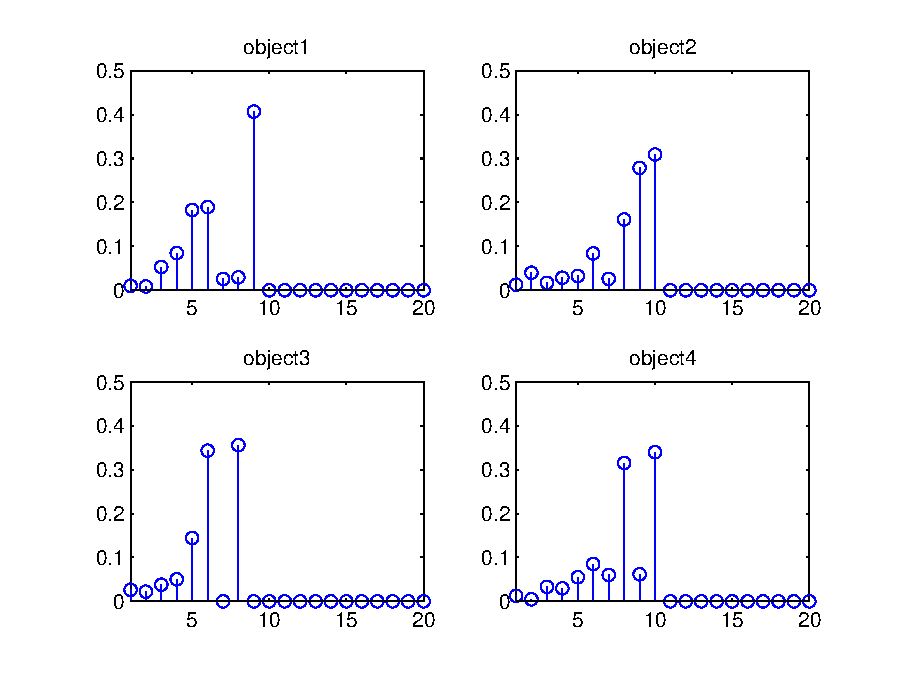
\includegraphics[width=11cm]{pecstrum_for_4objectinshadow1.eps}
	\caption{ Pectrum For Four Objects in "shadow1" image. }
	\label{fig:25}
\end{figure}

\begin{figure}
	\centering
	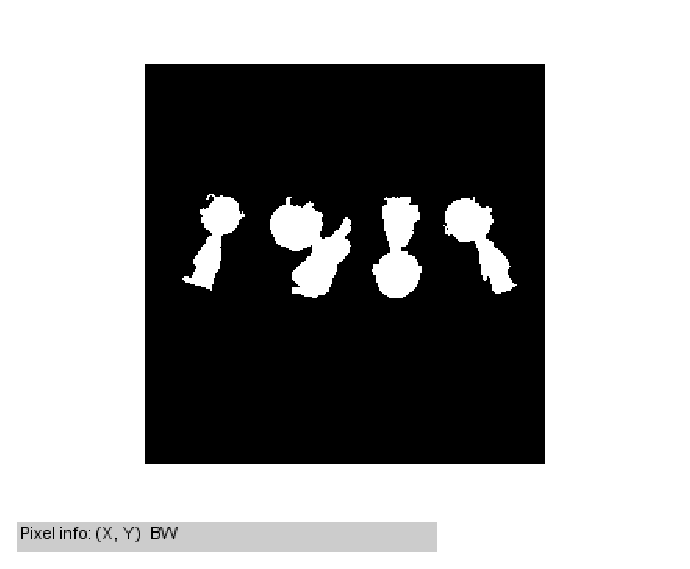
\includegraphics[width=11cm]{shadow1rotated_solidpart.eps}
	\caption{ Solid Objects in "shadow1rotated" image. }
	\label{fig:26}
\end{figure}





\begin{figure}
	\centering
	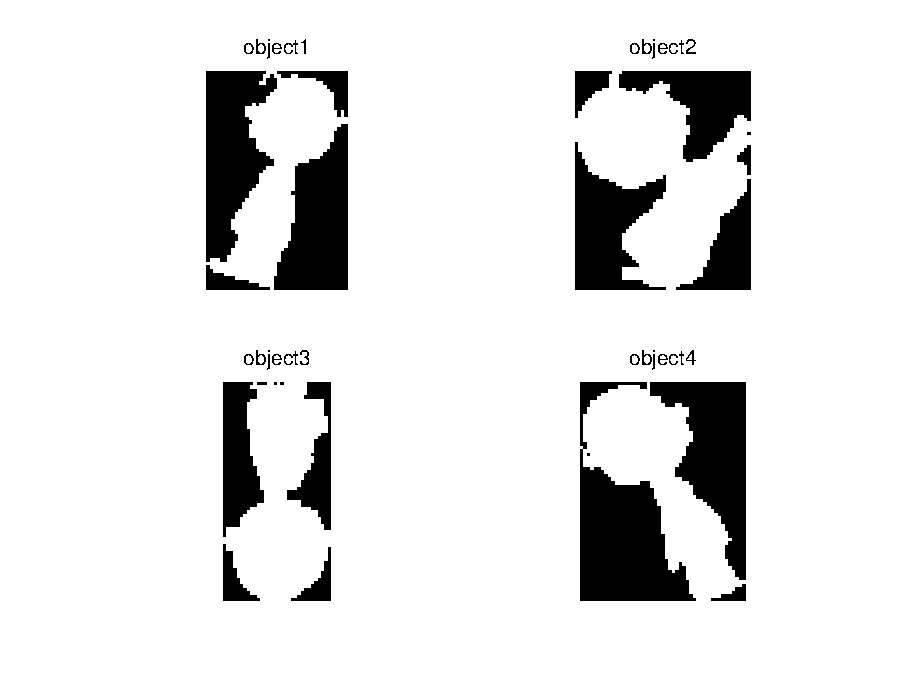
\includegraphics[width=11cm]{4objectinshadowrotated1.eps}
	\caption{ Four Objects in "shadow1rotated" image. }
	\label{fig:27}
\end{figure}

\begin{figure}
	\centering
	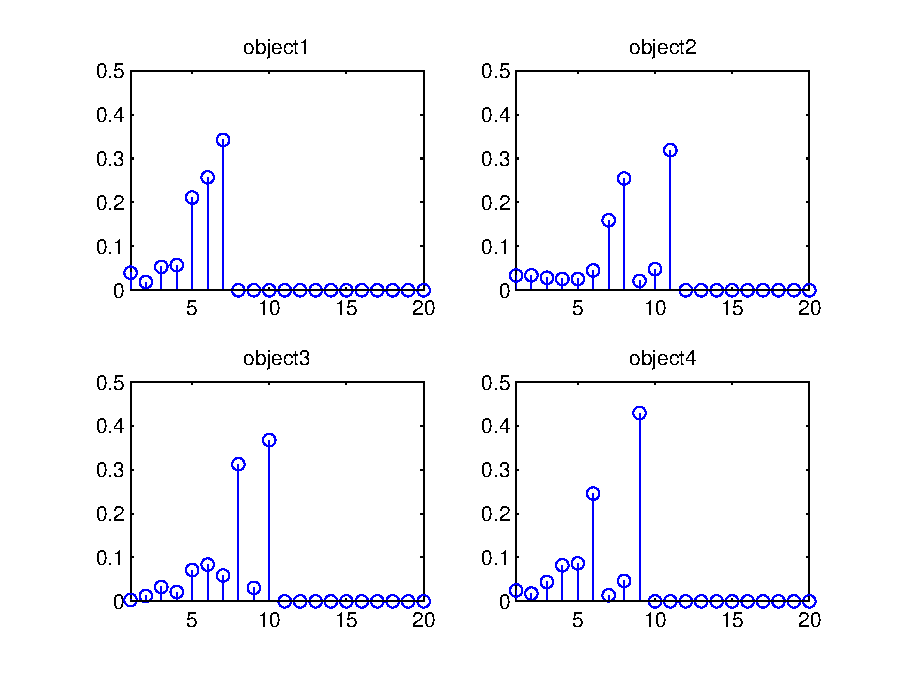
\includegraphics[width=11cm]{pecstrum_for_4objectinshadowrotated1.eps}
	\caption{ Pectrum For Four Objects in "shadow1rotated" image. }
	\label{fig:28}
\end{figure}





\subsection{ Discussion }

Note that we set all element in C as 1. Then, we got a result that two objects in "shadow1rotated" match to the same object in "shadow1". Specifically, object 2(ref2) and Object 3(ref3) in "shadow1rotated" are matched to object 4(ob4) in shadow1. In order to resolve this problem, we compared distances between ob4 and ref2 and between ob4 and ref3.  We found the distance between ob4 and ref3 is shorter,  and this means ob4 is best matched with ref3 not ref2. Finally, we found only object 2 (ob2) in "shadow1"  is not matched. We assumed ob2 matched with ref2. We proved this by comparing all distances between ob2 and objects (ref1~ref4) in "shadow1rotated" with the distance of the best matched pairs. Then, we found the distance between ob2 and ref1, the distance between ob2 and ref3, and the distance between ob2 and ref4, are not the shortest distance. Remove these choices, we got the result that ob2 is best matched with ref2.









\section{Conclusion}
To conclude our project, we implemented the conditional dilation in the first question. Also, the skeleton and partial reconstruction are applied in question 2. Furthermore, we computed the size distribution, pectrum, and complexity of each object.  Last, the member contributions are shown in Table~\ref{tab:contr}. We also want to thank professor Higgins for his lecture notes and hints.

\begin{table}
	\centering
	\caption{Member Contribution Summary}
	\begin{tabular}{c|c} \hline
       Su, Wei-Kai & experiments (1, 3) , report \\ \hline
	Kuo, Yu-Hsuan & experiment (2) ,report \\ \hline
	
	\end{tabular}
	\label{tab:contr}
\end{table}

\end{document}
